\section {User Manager}

\textit{User Manager} tab allow us on create,  modify or remove  account for/of users. Only user which possess privileges of administrator can manage of users accounts.

	\begin{figure}[!h] 
	\centering 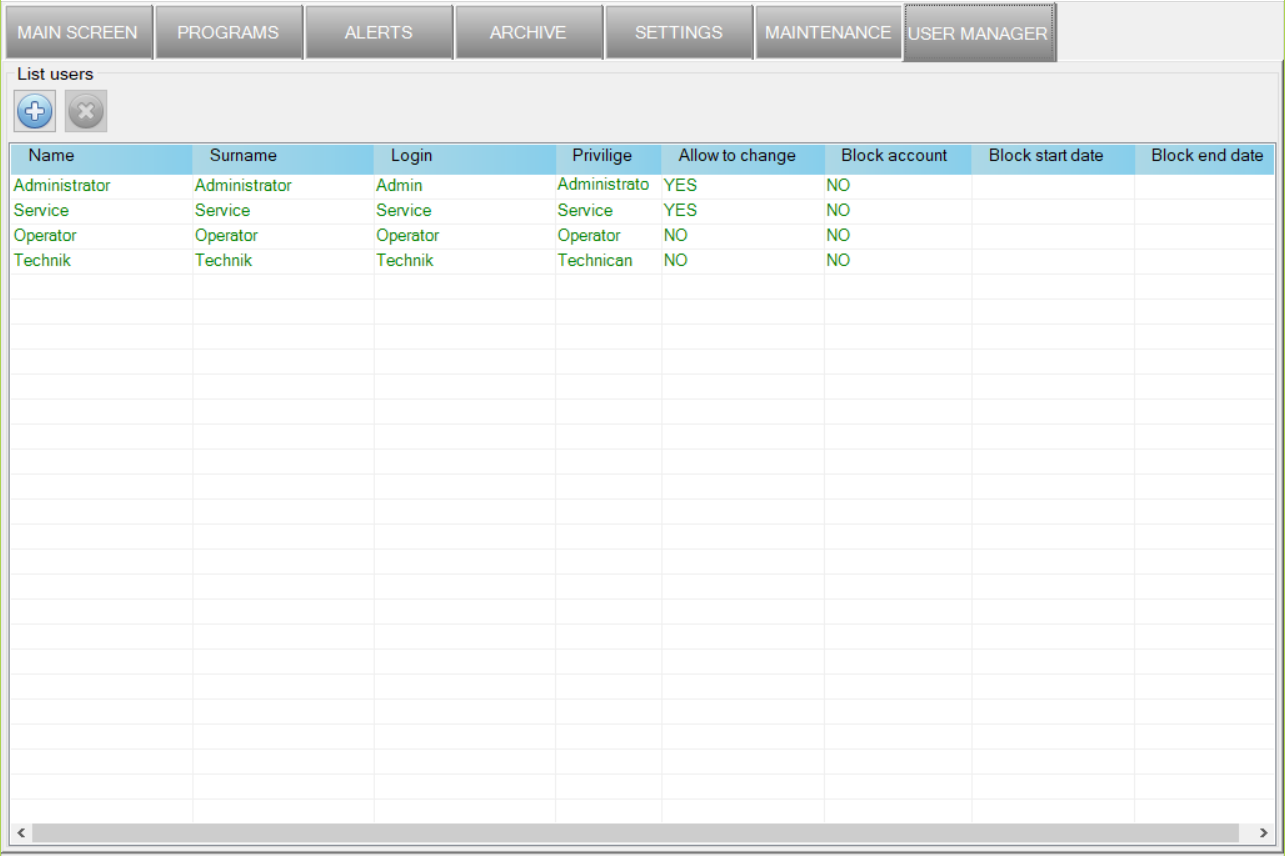
\includegraphics[width=0.8\textwidth]{Graphic/UserManager/UserMangerWindow.png}	
	\caption{User manager window}
	\label{user_mange_window}
	\end{figure}
	\FloatBarrier

To create or modify account of user we using below window.

	\begin{figure}[!h] 
	\centering 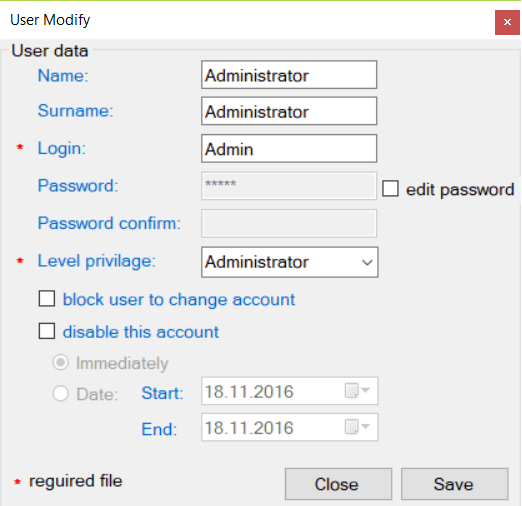
\includegraphics[width=0.5\textwidth]{Graphic/UserManager/UserModify.png}	
	\caption{User modify window}
	\label{user_ modify_window}
	\end{figure}
	\FloatBarrier

During create/modify account, administrator can define:

	\begin{itemize}
		\item \textit{Name} - name of user
		\item \textit{Surname} - surname of user
		\item \textit{Login} - login of user
		\item \textit{Password} - password to account
		\begin{itemize}
			\item \textit{block user to change account} - specify if user can modify password of this account
		\end{itemize}
		\item \textit{Privilige} - determine range of permission user to control of machine/application. We can select one of below options:
			\begin{itemize}
				\item \textit{Operator} - can control system in mode automatic
				\item \textit{Technican} - can control system in modes: manual and automatic
				\item \textit{Service} - can configured system
				\item \textit{Administrator} - can create/modify users accounta
			\end{itemize}
		\item \textit{Disable account} - specify if account should be disabled. Administrator has possibility disable account on two ways
		\begin{itemize}
			\item \textit{Immediately} - disable account from now
			\item \textit{Date} - disable account on defined date range  
		\end{itemize}
	\end{itemize}